{ %section2_4
	\subsection{Modification of Amdahl's law (according to Prof. Bukhanovsky)}
	\par In real computing systems, the OS spends resources on creating and deleting new threads. The time spent on these operations is not taken into account in Amdal's law. Parallel acceleration of $ S (p) $ depends on the number of cores and the proportion of parallelized operations, but does not depend on the number of the latter. We derive a formula in which the number of operations for which it is necessary to create a stream will be considered.
	\par Let $N$ be the number of parallelized operations, $ M $ be the number of non-parallelizable operations,  $t_c$ be the execution time of one operation, $p$ be the number of calculators (cores), $T_i$ be the program execution time using $i$ parallel threads on $i$ calculators, $\alpha$ is a certain scaling factor that encapsulates the amount of time required to create, delete a stream, and other overhead operations.
According to the Formula~\eqref{AmdalSFromP:equation}, $S(p)\;=\;\frac{T_1}{T_p}$.
	\par First we find $ T_1 $. Since this code is linearly executed, the time spent on its execution will be equal to the number of operations times the time it takes to execute one operation: $T_1\;=\;t_c(N\;+\;M)$. 
	\par The execution time of the parallel $T_p$ program includes the time to create the stream: $t_c\alpha(p\;-\;1)N$ need to create $(p\;-\;1)$ new threads, since the main thread has already been created and for each spend some time $\alpha$),  $\frac {t_cN}p$ parallel code running time on all cores: $t_cM$. Total, dividing $T_1$ на $T_p$, we get the formula of Amdahl’s law according to prof. Bukhanovsky:
	\begin{equation}
		\label{AmdalBuhunovsky:equation}
		S(p,N)\;=\;\frac{T_1}{T_p}\;=\;\frac{N\;+\;M}{\alpha(p\;-\;1)N\;+\;\frac Np\;+\;M}
	\end{equation}
From the Formula~\eqref{AmdalBuhunovsky:equation} we can see that with an increase in the number of cores after a certain limit $S(p,N)$ will not grow as in Amdahl’s law, since time will be spent a lot of time creating new threads. On the Figure~\ref{GraphAmdalBuhunovsky:image} it is clearly seen that $S(p,N)$ decreases with a large number of threads and becomes noticeably smaller $S(p)$ than Amdahl even with a small value $\alpha$.
	\begin{figure}[H]
		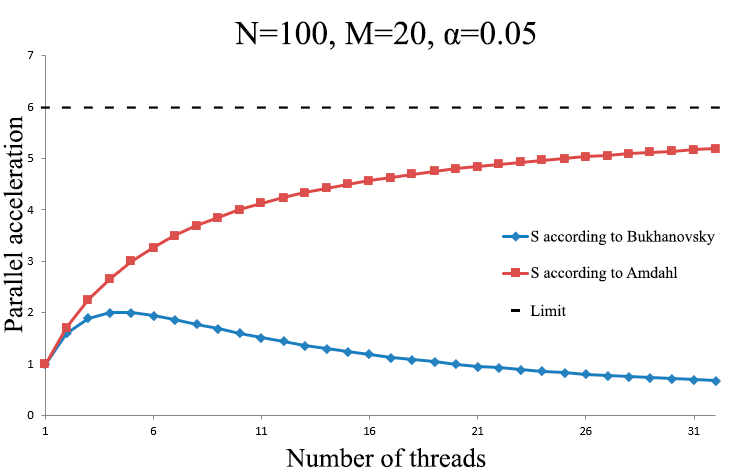
\includegraphics[width=1\linewidth]{GraphAmdalBuhunovsky}
		\caption{\textit{Graph of parallel acceleration versus number of threads}}
		\label{GraphAmdalBuhunovsky:image}
	\end{figure}
}